\part{Algorithms} \label{part:three algorithms}

\chapter{T-distributed Stochastic Neighbor Embedding (T-SNE)}

\section{Background}

some related work and background

\section{Asymmetric SNE}

Given N observations of some high dimensional data, for any pair, $x_i$ and $x_j$, SNE defines the similarity (aka an affinity or weight) between them, using a Gaussian kernel function:

\begin{equation*}
    {v_{j\mid i}} = \exp {(-\beta_i r^2_{ij})} 
\end{equation*}

\noindent Where $r_i_j$ is the distance between $x_i$ and $x_j$ and $\beta_i$ must be determined by some method. The notation of $v_{i \mid j}$ rather than $v_i_j$, is to indicate that this quantity is not symmetric, i.e. $v_{i \mid j} \neq v_{j \mid i}$. This notation is from the conditional versus joint probability definitions used in symmetric SNE (see below). The $r_i_j$ notation indicates that the distances are symmetric.\\

\noindent The weights are normalized to form $N$ probability distributions:

\begin{equation*}
    {p_{j\mid i}} = \frac {v_{j\mid i}} {\sum_k^N v_{k\mid i}}
\end{equation*}

\noindent $\beta_i$ is chosen by finding that value that results in the probability distribution having a specific perplexity. The perplexity has to be chosen by the user, but is interpreted as being a continuous version of the number of nearest neighbors, and generally is chosen to take values between 5 and 50. $p_{j\mid i}$ is a conditional probability, and is interpreted as the probability that item j will be chosen as being similar to item i, given that item i was picked already.

\noindent At the same time, the output space of the embedded coordinates, which is the similarity between the points $y_i$ and $y_j$ is also defined as a Gaussian:

\begin{equation*}
    {{w_i_j} = \exp {(-d^2_{ij})} }
\end{equation*}

\noindent $d_i_j$ is the Euclidean distance between $y_i$ and $y_j$ as the mapping points of high-dimensional data points $x_i$ and $x_j$ in low-dimensional space, respectively. There is no $\beta$ in this weight definition so these weights are symmetric. The output probabilities, $q_{j\mid i}$ are calculated from $w_i_j$ in the same way that we go from ${v_{j\mid i}}$ to ${p_{j\mid i}}$, again creating N probability distributions. Due to normalizing by rows, the $q_{j\mid i}$ are asymmetric despite the symmetric weights they are generated from.\\

\noindent Therefore, The SNE cost function could be defined as the sum of the Kullback-Leibler divergences of the N distributions:

\begin{equation*}
    {C_S_N_E} = {\sum_i KL(P_i \mid \mid Q_i)} =  { {\sum_i^N} {\sum_j^N} {p_{j\mid i}} \log \frac{p_{j\mid i}}{q_{j\mid i}} }
\end{equation*}

\noindent The gradient of $y_i$ of the SNE cost function is as follows:

\begin{equation*}
\frac{\partial C_{SNE}}{\partial y_i} = 2\sum_j(p_{j \mid i} - q_{j \mid i} + p_{i \mid j} - q_{i \mid j} )(y_i - y_j)
\end{equation*}

\noindent Because KL distance is an asymmetric scale. The purpose of minimizing the cost function is to make the values of $p_{j∣i}$ and $q_{j∣i}$ as close as possible,  that is, the similarity of points in the low-dimensional space is consistent with the similarity of points in the high-dimensional space. But it can be trimmed from the form of the cost function. When $p_{j∣i}$ is relatively bigger and $q_{j∣i}$  is relatively smaller, the cost is higher; when $p_{j∣i}$ is smaller and $q_{j∣i}$ is bigger, the cost is lower. This means when two data points in a high-dimensional space are relatively close, if they are mapped to a low-dimensional space and are farther apart, then they will get a high penalty, which is of course no problem. Conversely, when the two data points in the high-dimensional space are farther apart, if they are mapped to the low-dimensional space, they will get a very low penalty value. This is a problem, and it should be a higher penalty. In other words, the cost function of SNE pays more attention to the local structure rather than global impact.

\section{Symmetric SNE}
In Symmetric SNE, the input probability matrix is symmetrized by averaging pj|i and pi|j and then re-normalized over all pairs of points, to create a single (joint) probability distribution, $p_i_j$:

\begin{equation*}
    {p_{i j}} = \frac {p_{i\mid j} + p_{j\mid i}} {2N}
\end{equation*}

\noindent The output probabilities, $q_i_j$ are now defined by normalizing the output weights over all pairs, again creating a single probability distribution:

\begin{equation*}
    {q_{i j}} = \frac {w_{i j}} {\sum_k^N \sum_l^N w_{k l}}
\end{equation*}

\noindent Where $N$ is the total number of data points, this definition not only satisfies the symmetry, but also ensures that the penalty value of xi will not be too small. Which maens no matter where the outlier's mapping point in low dimension $y_i$ in the space is at any position, the penalty value can be guaranteed. At this time, the following cost function can be written using KL distance:

\begin{equation*}
    {C_S_S_N_E} = {\sum_i KL(P \mid \mid Q)} =  { {\sum_i^N} {\sum_j^N} {p_{i j}} \log \frac{p_{i j}}{q_{i j}} }
\end{equation*}

\noindent The gradient turn out to be: 

\begin{equation*}
\frac{\partial C_{SSNE}}{\partial y_i} = 4\sum_j(p_i_j - q_i_j)(y_i - y_j)
\end{equation*}

\noindent In the end, the result for UPS database, which has five kind of image of hand writing can be seen as below:

% \begin{figure}[ht]

% \centering
% 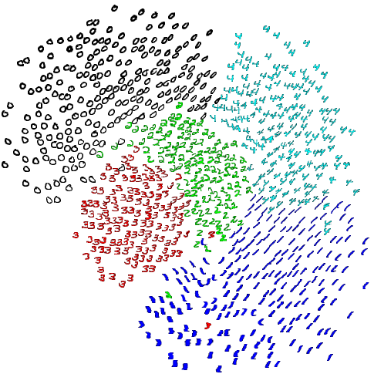
\includegraphics[scale=1.5]{images/image_SNE.png}
% \caption{result of SNE algorithm for UPS dataset}
% \label{fig:label}
% \end{figure}

\section{The Crowding Problem}

As we can observe from the image above, the dimension reduction result is satisfied, which means different kinds of images can be clustered by each category. However, the boundary between each cluster is not clear enough. It would be hard to tell the difference if there is no marks in different color for each group, which is also not convenient for data visualization.\\  

\noindent Part of the reason of this situation is the SNE algorithm pays more attention to the local structure than the global structure. The more important reason could be the difference between the high-dimensional space distance distribution and the low-dimensional space distance distribution. With the increase of the dimensions, the sparseness of high-dimensional spatial data will also increase because the volume increases exponentially.\\

\noindent If there is An $m$-dimensional sphere with radius $r$ centered on data point $x_i$, its space increase with $r^m$. Assuming that the data points are uniformly distributed in the m-dimensional sphere, The distance between other data points and $x_i$ as the dimension increases could be observed as below:

\begin{figure}[ht]

\centering
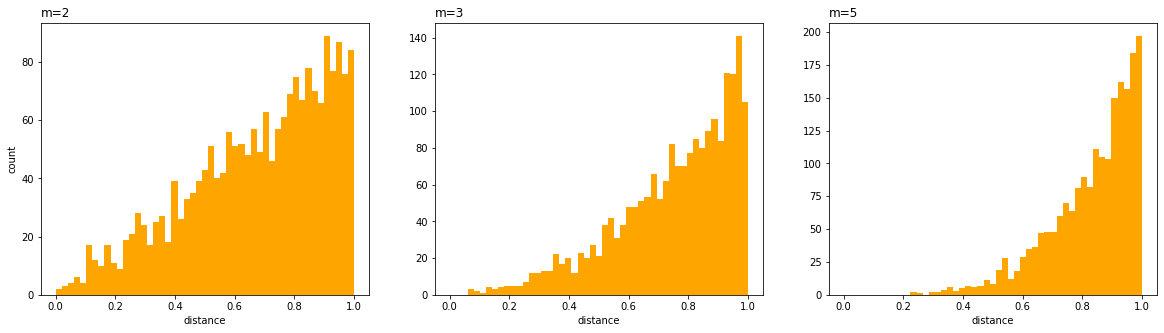
\includegraphics[scale=0.34]{images/image_crowding_problem_1.png}
\caption{distribution of distances between $x_i$ with dimension 2 to 5}
\label{fig:label}
\end{figure}

\begin{figure}[ht]

\centering
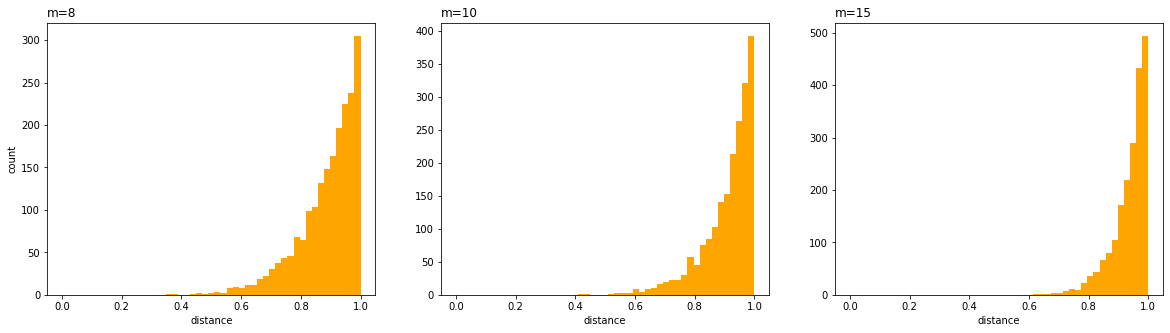
\includegraphics[scale=0.34]{images/image_crowding_problem_2.png}
\caption{distribution of distances between $x_i$ with dimension 8 to 15}
\label{fig:label}
\end{figure}

\noindent It can be observed from the figure that as the dimension increases, most of the data points are clustered near the surface of the sphere, and the distance distribution from the point $x_i$ is extremely uneven. If this distance relationship is directly retained to a low dimension, there will be a crowding problem.

\section{T-SNE}
Draw a random sample with a capacity of $N$ from the normal population. If the mean of the normal population is $μ$, the variance is $\sigma^2$. The mean of the random sample is $\bar{x}$, and the variance is $s^2=  \frac {1}{N−1} \sum ^N_{i=1} (x_i−\bar{x})^2$, and the random variable t can be expressed as:

\begin{equation*}
    {t} =  \frac {\bar{x} - \mu}{s / \sqrt{N}} 
\end{equation*}

\noindent $t$ satisfies the t distribution with n−1 degrees of freedom, written as, $t∼t(n−1)$. t distribution is a typical long-tailed distribution. It is relatively gentle at both ends of the tail, which has obvious advantages when dealing with small samples and abnormal points.\\

\begin{figure}[ht]

\centering
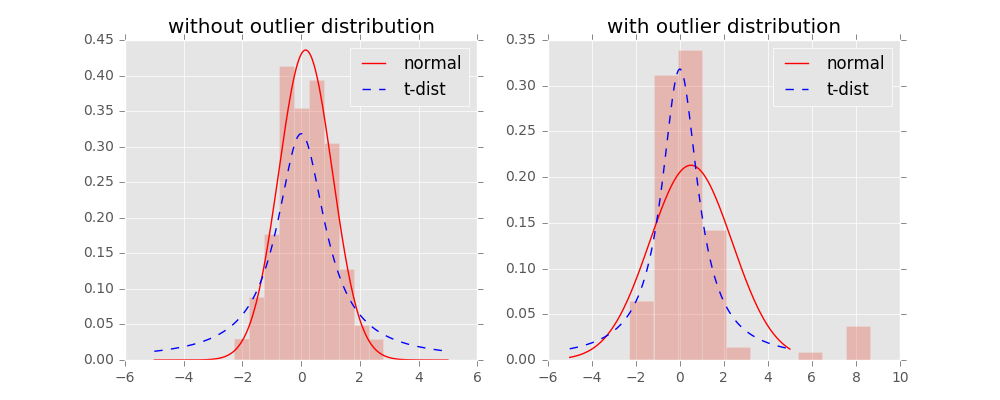
\includegraphics[scale=0.6]{images/image_t-distribution.png}
\caption{normal distribution and t distribution with and with out outliers}
\label{fig:label}
\end{figure}

\noindent From the figure 2.3, it can be easily observed that when there are no outliers, the fitting result of t distribution and Gaussian distribution are basically consistent. In the second picture, there are some abnormal points. Because the tail of the Gaussian distribution is low, it is more sensitive to abnormal points. In order to take care of these abnormal points, the fitting result of the Gaussian distribution deviates from the location of most samples, and the variance is also large. In contrast, the tail of the t distribution is relatively high and it is not sensitive to outliers, that ensure its robustness, so its fitting results are more reasonable, and the overall characteristics of the data are better captured.\\

\noindent With the t distribution now, for points that are close in high-dimensional space, in order to satisfy $p_i_j$=$q_i_j$, the distance in low-dimensional space needs to be slightly smaller; and for points that are far apart in high-dimensional space, in order to satisfy $p_i_j$=$q_i_j$, in low-dimensional space The distance needs to be farther. Then, We redefine the weight function from symmetric SNE: 

\begin{equation*}
    {w_i_j} =  \frac {1}{1+d_i_j^2} 
\end{equation*}

\section{Barnes-Hut t-SNE(BH t-SNE)}

BH t-SNE has some improvements comparing with t-SNE algorithm with the help of tree-based algorithm, including two parts: one is the use of kNN graphs to represent the similarity of points in the high-dimensional space; the other is the optimization of the gradient solution process. The gradient calculation is divided into two parts of gravity and repulsion, and some optimization techniques are also used.

\subsection{kNN graph for the similarity in HD space}

\noindent In t-sne, the overall distance distribution relationship in the high-dimensional space is expressed in the following form:

\begin{equation*}
    {v_{j\mid i}} = \exp {(-\beta_i r^2_{ij})} 
\end{equation*}

\begin{equation*}
    {p_{j\mid i}} = \frac {v_{j\mid i}} {\sum_k^N v_{k\mid i}}
\end{equation*}

\begin{equation*}
    {p_{i j}} = \frac {p_{i\mid j} + p_{j\mid i}} {2N}
\end{equation*}\\

\noindent These three formulas means every data point need to calculate the variance considering all other points. But in fact, the probability $p_i_j$ that two distant points are neighbors to each other is very small and almost negligible. This makes the efficiency of t-SNE is significantly reduced when processing large-scale high-dimensional data.\\

\noindent Therefore, when constructing a distance similarity relationship for a point in a high-dimensional space, it is not necessary to consider every node in the graph, only a number of similar nodes. Here we consider the ⌊3$u$⌋ points closest to the point $x_i$, where $u$ is the perplexity of the conditional probability distribution around the point $x_i$, and only consider the set of these points, which will decrease the amount of calculation. The BH t-SNE algorithm uses a VP tree (vantage-point tree) to construct this kNN graph, and an accurate kNN graph can be obtained within O ($uNlogN$) time complexity.\\

\subsection{Approximation of repulsion in gradient}

When understanding the physical meaning of t-SNE gradient, the gradient can be regarded as the resultant effect of all other points on $y_i$. If $Z$ is set as $Z = \sum_{k \neq l} (1+ \mid y_k−y_l \mid ^2)^{-1}$, then the gradient could be transformed by this feature:

\begin{equation*}
\begin{aligned}
\frac{\partial C_{SSNE}}{\partial y_i} &= {4\sum_j(p_i_j - q_i_j)(y_i - y_j)(1 + \mid y_i - y_j \mid ^ 2) ^{-1}}\\
&= {4\sum_j(p_i_j - q_i_j) (1 + \mid \mid y_i - y_j \mid \mid ^ 2)}
\end{aligned}
\end{equation*}

\begin{equation*}
\begin{aligned}
\frac{\partial C_{SSNE}}{\partial y_i} &= {4(F_{attraction} + F_{repulsion})}\\
&= 4({\sum_{i \neq j}p_i_j q_i_j Z (y_i - y_j)} - {\sum_{i \neq j}q_i_j^2 Z (y_i - y_j)}) 
\end{aligned}
\end{equation*}

\noindent It can be seen that after decomposing the gradient into two parts of attraction and repulsion, the first part is easier to calculate since the $q_i_j Z = 1 + \mid y_i - y_j \mid ^ 2 $ could use the approximation above, which only considers the nearest neighbor nodes, while ignoring distant nodes with time complexity is $O(uN)$. However, there is still a large amount of calculation to calculate repulsion with time complexity $O(N^2)$ because the distribution of $P$ and $Q$ is different, but there are still some optimization techniques to simplify this calculation.\\

\noindent If there are three data points ($y_i,y_j,y_k$) as shown below, their distance relationship can be summarized as $y_i−y_j ≈ y_i−y_k >> y_j−y_k$, the repulsion of $y_j$ and $y_k$ to $y_i$ is approximately equal.

\begin{figure}[ht]

\centering
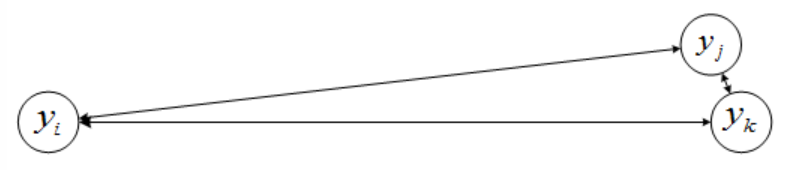
\includegraphics[scale=0.6]{images/image_point_region_1.PNG}
\caption{normal distribution and t distribution with and with out outliers}
\label{fig:label}
\end{figure}

\noindent This situation is very common in low-dimensional space, and even the repulsive force of each point in a certain area can be approximated by the same value. If a point is given arbitrarily, we just need to calculate the repulsion between given point and the centroid of the data points within the certain area, and use the optimization method just now to calculate the total repulsion for them. Of course, not all regions meet this approximate condition. Here, the Barnes-Hut algorithm is used to search and verify the point-region pairs that meet the approximate condition.\\

\subsection{From point-area to area-area}

\noindent In the above approximation, we consider the approximation of the repulsive force between a point and an area. In fact, we can further optimize and consider the approximation of the repulsive force between one area and another area.
\\

\begin{figure}[H]
\centering  %图片全局居中
\subfigure[name1]{
\label{Fig.sub.1}
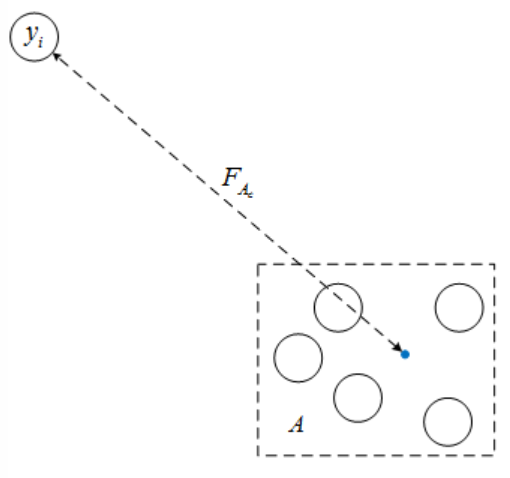
\includegraphics[width=7cm,height=5cm\textwidth]{images/image_point_region_2.PNG}}
\subfigure[name2]{
\label{Fig.sub.2}
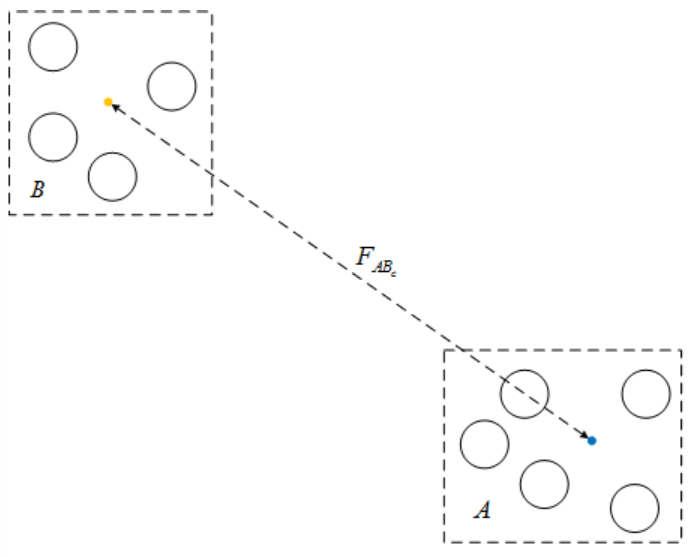
\includegraphics[width=7cm,height=5cm\textwidth]{images/image_region_region_1.PNG}}
\caption{Main name}
\label{Fig.main}
\end{figure}

\noindent Since the result from these two algorithm have similar accuracy and Barnes-Hut T-SNE is much faster than another. This thesis will focus the performance and characteristics of it.

% 再补两个通过bh t-SNE 和 t-SNE 的效果图

\chapter{LargeVis}



\noindent  Although T-SNE works well on small-scale data, there are still some disadvantages of T-SNE:\\

\noindent 1. The efficiency of t-SNE is significantly reduced when processing large-scale high-dimensional data (including BH T-SNE)\\

\noindent 2.The parameters of t-SNE are sensitive to different data sets, which means that even finding out the proper parameters setting for T-SNE in one data set with there is a good visualization effect. However, it cannot be applied to another data set, and it takes a lot of time to find new suitable parameters.\\

\noindent As can be seen from the name, the goal of LargeVis\cite{ref5} is the visualization of large-scale data sets, which takes a different approach comparing with T-SNE: it reuses many of the same definitions as t-SNE but makes sufficiently modified so that stochastic gradient descent can be used. The main improvement is the efficient algorithm for constructing kNN graphs, as well as the low-dimensional space probability calculation formula and objective function.

\section{Efficient kNN graph constructing algorithm}

In the BH t-SNE, for high-dimensional spatial distance similarity, it only consider several neighbor points closest to $x_i$, which is essentially a process of constructing a kNN graph. The VP(vantage-point) tree is used to construct an accurate kNN graph, but the efficiency is still not good, especially for the large-scale dataset. And LargeVis uses a more ingenious way, instead of pursuing a one-step approach, first approximate and then improve accuracy.\\

\subsection{K-D tree and Random Projection Tree}

There are generally three types of common methods for building KNN graph: the first type is the space-partitioning trees algorithm, the second type is the locality sensitive hashing algorithm, and the third type is the neighbor exploring techniques algorithm. Among them, k-d tree and random projection tree belong to the first type of algorithm.\\

\noindent A k-d tree is a data structure that partitions a k-dimensional data space, and is essentially a binary tree. It is mainly used for searching key data in multi-dimensional space, such as range search and nearest neighbor search. The following figure shows the use of k-d trees to search for k nearest neighbors in a two-dimensional space, and then construct a kNN graph. It constructs a kd tree through a recursive process. The root node corresponds to all points in the area. After dividing the space into a left subtree and a right subtree in a certain dimension, the next level of child nodes can be obtained by repeating the splitting process of the root node. Until the number of points corresponding to all leaf nodes in the kd tree is less than a certain threshold.\\

\begin{figure}[ht]

\centering
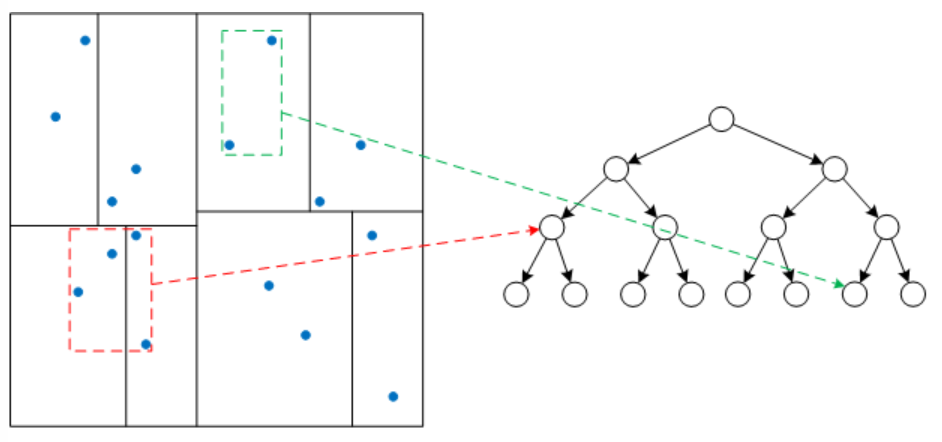
\includegraphics[scale=0.85]{images/image_largevis_k-d_tree_1.PNG}
\caption{k-d tree for dimension 2}
\label{fig:label}
\end{figure}

\noindent With the k-d tree, we don't have to calculate the distance between a certain point and all other points one by one to find k nearest neighbors. For example, to find the k-nearest neighbors of the red dot in the figure below, it only need to search the current subspace, and at the same time, continue to backtrack and search other subspaces of the parent node to find the k-nearest neighbors.\\

\begin{figure}[ht]

\centering
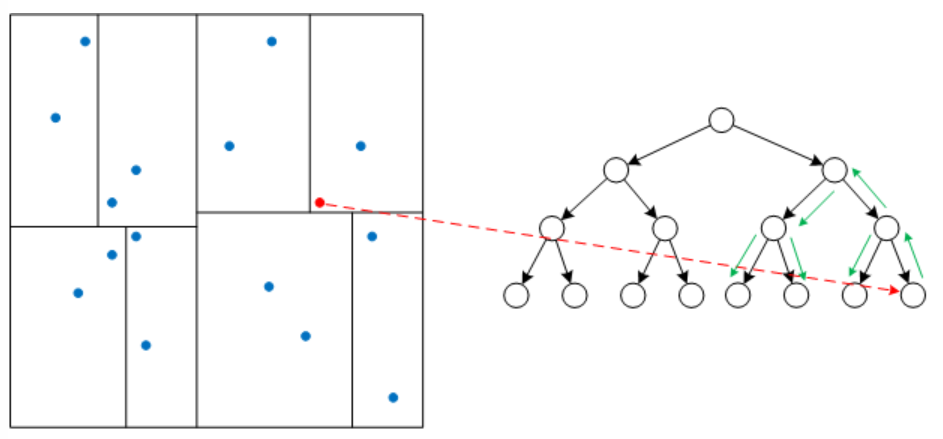
\includegraphics[scale=0.85]{images/image_largevis_k-d_tree_2.PNG}
\caption{finding k-nearest neighbors for k-d tree}
\label{fig:label}
\end{figure}

\noindent However, the biggest problem with the k-d tree is that the way it divides the space is relatively rigid, which is strictly based on the coordinate axis. For high-dimensional data, each dimension of the high-dimensional data is used as a coordinate axis. When the data dimensionality is high, the depth of the k-d tree could be a lot also, which may also lead to the dimensionality disaster problem.\\

\noindent In contrast, the way of dividing the space by random projection trees is more flexible. The basic idea of the random projection tree is similar to the k-d tree, but the way to divide the space is not according to the coordinate axis, but according to the randomly generated unit vector. Because the data in principle is on a manifold, instead of a disorderly manner. Therefore, the depth of the random projection tree is not determined by the dimensionality of the data, but depends on the dimensionality of the manifold where the data is located\cite{ref6}.\\

\begin{figure}[ht]

\centering
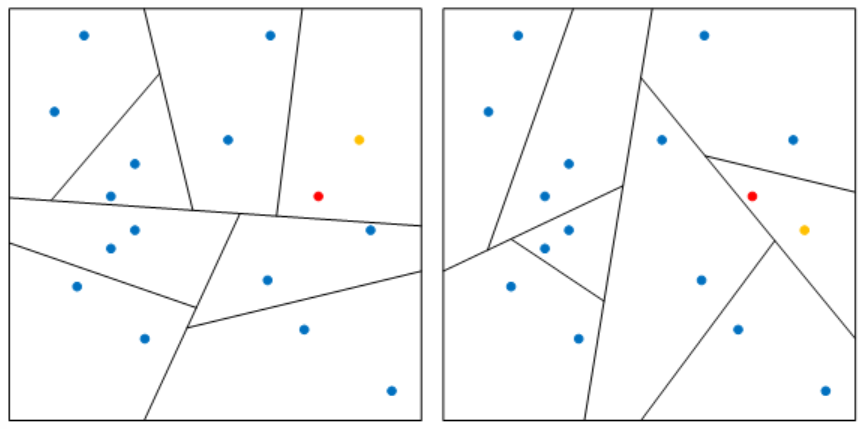
\includegraphics[scale=0.85]{images/image_largevis_random_projection_tree_2.PNG}
\caption{finding k-nearest neighbors for random projection tree}
\label{fig:label}
\end{figure}

\noindent When a random projection tree is used to find k nearest neighbors, the backtracking search method is similar to the k-d tree. If the requirement of the tree's accuracy is not high, the characteristics of the random projection tree can be used to adopt a simpler and time-saving method. That is, we can construct multiple random projection trees in parallel. Since the divided unit vectors are generated randomly, each random projection tree divides the current space differently, as shown in the following figure with two-dimensional space as an example. If the k-nearest neighbors of the red dot need to be fixed, it only need to search the subspace where it is located in different random projection trees, and finally take the union. Although this is time-consuming and space-consuming in the process of constructing a random projection tree, it is very efficient in the search phase.

\subsection{The neighbor’s neighbor may also be my neighbor}

The idea of "neighbors' neighbors may also be my neighbors", starting from an initial nearest-neighbor graph, the algorithm iteratively refines the graph by exploring the neighbors of neighbors defined according to the current graph\cite{ref5}. It use the neighbor search algorithm to find potential neighbors, calculating the distance between the neighbor and the current point, the neighbor's neighbor and the current point, and putting them into a small root pile. Take the k nodes with the smallest distance as k nearest neighbors, and finally get an accurate kNN graph.\\

\section{Low-dimensional space visualization algorithm}

\noindent After completing the KNN graph algorithm for high dimensional space, we need to project the nodes of the graph into a low-dimensional space. In the process of low-dimensional space visualization, the idea of t-SNE is to ensure that the distance distribution P of the high-dimensional space and the distance distribution Q of the low-dimensional space are as close as possible, and use the KL distance to write the cost function and find the gradient. But the efficiency problem has not been solved well.\\

\noindent In LargeVis algorithm, in order to solve the efficiency problem, a probability model is applied to it to maintain the similarity of vertices in low-dimensional space. That is, the algorithm will bring similar vertices close to each other in a low-dimensional space, and separate different vertices from each other. It uses two models from Word2vec and negaitve sampling optimization method to 
achieve the goal.

\subsection{Word2vec and Negative sampling}
Word embedding is a way to present word using numerical representation in order to understand the contextual meaning of the words, While word2vec provide two kind of architectures 1)Continuous Bag of-Words (CBOW) and 2)Skip-gram and combine with two methods 1)negative sampling and 2)hierarchical softmax method to obtain this representation way of each word. Skip-gram: works well with a small amount of the training data, represents well even rare words or phrases. CBOW: several times faster to train than the skip-gram, slightly better accuracy for the frequent words.

\subsubsection{Two models of Word2vec}

\noindent As we can see from the figure 3.4, the CBOW method, the surrounding words are used to predict the center word, so as to use the prediction result of the center word, use the Gradient Desent method to continuously adjust the vector of the surrounding words. When the training is completed, each word will be used as the central word, and the word vectors of the surrounding words are adjusted, so that the word vectors of all words in the entire text are obtained. The CBOW model performs better with a small amount of training data, and is more suitable for rare words or phrases.\\

\begin{figure}[ht]

\centering
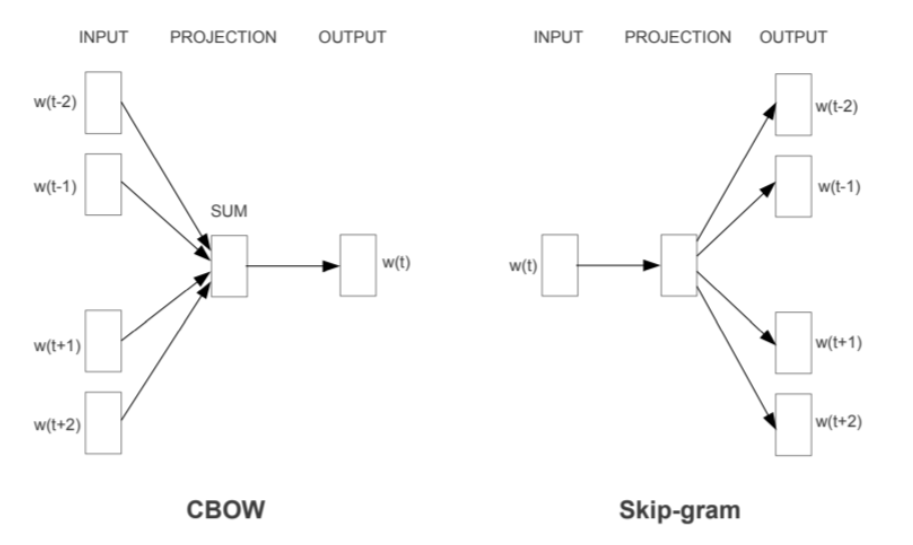
\includegraphics[scale=0.85]{images/image_largevis_word2vec.PNG}
\caption{Two models of Word2vec}
\label{fig:label}
\end{figure}

\noindent The Skip-gram uses the head word to predict surrounding words. In skip-gram, the prediction results of surrounding words are used, and Gradient Decent is used to continuously adjust the word vector of the central word. After all the text is traversed, the word vectors of all words in the text are obtained. The Skip-gram model is faster to train and is more suitable for frequent words or phrases.\\


\subsubsection{Negative sampling}

\noindent Negative sampling is one of the optimization techniques. If we take the Skip-gram model as an example. The idea of the Skip-gram model is to predict the context from the target word and use a context window to limit the text range. It needs to maximize the probability that the context window appears around the target word.That is to maximize $p(c∣w)=∑p(wi∣w)$. The words $w_i ∈ c$ that appear in the context window around the target word constitute a positive sample $(wi, w)$, and the words $w_j ∈ D$ that do not appear around the target word constitute a negative sample $(w_j, w)$ and the goal of this step is to maximize the probability of positive samples during the training process, while also reducing the probability of negative samples.\\

\noindent Due to the large number of negative samples (words outside the context window can basically constitute negative samples), it is obviously unrealistic to directly consider all negative samples, so we can select a part of negative samples by sampling. Because some words appear frequently in the corpus and some words appear low, it is obviously not advisable to draw negative samples directly from the vocabulary. Word2vec uses a weighted sampling strategy, that is, sampling according to word frequency. High-frequency words are more likely to be sampled, and low-frequency words are less likely to be sampled.\\

\begin{figure}[ht]

\centering
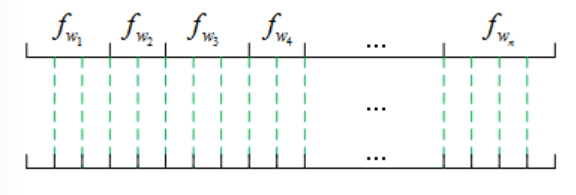
\includegraphics[scale=1.3]{images/image_largevis_word2vec_seperate_lines.PNG}
\caption{Weighted sampling details}
\label{fig:label}
\end{figure}

\noindent As we can see in figure 3.5, the upper line segment is divided by word frequency, the higher the word frequency, the longer the line segment, and the lower line segment is divided equally. We randomly place dots in the lower line segment (uniformly distributed), and according to the interval where the point falls, correspond to the upper line segment to determine the word sampled. Intuitively, in this way, words with higher word frequency are more likely to be sampled, and words with lower word frequency are less likely to be sampled.After adding negative sampling optimization, the form of the objective function becomes:

\begin{equation*}
    {log \sigma(v_{w_c}^T \cdot v_w)} + {\sum^k_{\substack{i=1\\ {E_{w_i} \sim P_n(f)}}}log \sigma(-v_{w_c}^T \cdot v_w)}
\end{equation*}

\noindent Where $w$ represents the target word, $w_c$ represents the word in the context window around the target word (positive sample), $w_i$ represents the word that does not appear in the context window (negative sample), $k$ represents the number of negative samples extracted, and $P_n(f)$ is Used for noise distribution generated by negative samples, $f$ represents word frequency, $P_n(f)∝f^{0.75}$. The exponent is suggested to set as 0.75\cite{ref7}, this makes the data closer to the center, which means the 
higher values tend to lower and the lower values do the opposite in order to avoid high frequent words appearing all the time.

\subsection{Large-scale Information Network Embedding (LINE) and edge-sampling algorithm}

\noindent There are mainly two outstanding contributions for LINE: one is that it can adapt to various types (undirected edges or directed edges, weighted and unweighted) large-scale (million-level nodes, billion-level edges) networks, and can It captures the first-order and second-order similarities in the network very well; the second is to propose a very powerful edge-sampling algorithm, which greatly reduces the time complexity of LINE. After using the edge-sampling algorithm, the time complexity and The number of edges in the network is linear. The efficiency of LargeVis also benefits from LINE and its edge sampling algorithm.\\

\noindent The first-order similarity refers to the point-to-point similarity between two nodes in the network, specifically the weight of the edge between the nodes (if the point does not have an edge, the first-order similarity is 0); the second-order similarity Sex means that if nodes share similar neighbor nodes, then the two tend to be similar. For example, in the case shown in the figure below, the weight of the edge is expressed in thickness:

\begin{figure}[ht]

\centering
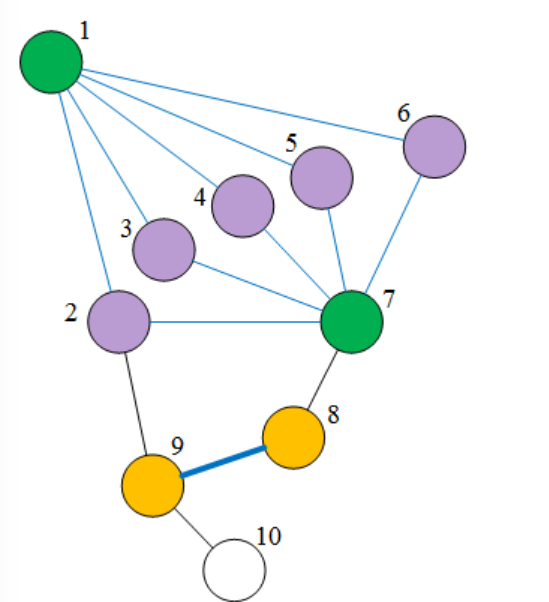
\includegraphics[scale=0.85]{images/image_largevis_line_1.PNG}
\caption{edge sampling example}
\label{fig:label}
\end{figure}

\noindent The first-order similarity between node 8 and node 9 in the graph is higher because the weight of the directly connected edges is higher. Node 1 and node 7 have most of the same neighbors, so the second-order similarity between the two is very high. The idea of edge sampling algorithm comes from the negative sampling optimization technique used by Mikolov in word2vec. It not only improves the efficiency of training, but also solves the problem of sharp increase in gradient caused by the weighted edge in the network representation during the training process.\\

\subsection{Visualization algorithm}

\noindent The application of negative sampling to words is mentioned above. In fact, it is similar in the network. We can regard the current center point as the target word, and its neighbor nodes as words appearing in the context window, then the center point and its neighbor nodes That is, it constitutes a positive sample, while the center point and non-neighboring points constitute a negative sample.

\begin{figure}[ht]

\centering
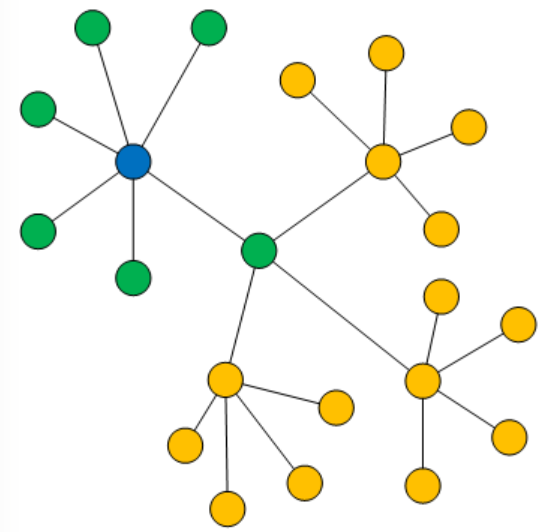
\includegraphics[scale=0.85]{images/image_largevis_ld_visulization_1.PNG}
\caption{edge sampling example}
\label{fig:label}
\end{figure}

\noindent As a small part of the kNN diagram shown above, if the blue point is the center point, each green point and the blue point can form a positive sample, and each yellow point and the blue point form a negative sample. How to map the structural relationship in this kNN graph to a low-dimensional space? Intuitively, in the low-dimensional space, the node pairs in the positive sample should be clustered together, while the node pairs in the negative sample are scattered far away. Let us first consider the case of a weightless network. Use $y_i$ and $y_j$ to represent two points in a low-dimensional space. The probability that the two points have a binary edge $e_i_j=1$ (the edge with weight 1) in the kNN graph is:

\begin{equation*}
    P(e_i_j = 1) = f( {\mid \mid y_i - y_j \mid \mid} ^ 2)
\end{equation*}

\noindent Among them, f(⋅) similarly uses th e$t$ distribution in t-SNE, $f(x)= \frac{1}{1+x^2}$, if the distance between $y_i$ and $y_j$ is smaller, the probability of two points having a binary edge in the kNN graph is higher On the contrary, if the distance between $y_i$ and $y_j$ is larger, the probability that two points have binary edges in the kNN graph is smaller. LargeVis also considers the weighted network, and defines the probability that the edge weight is $w_i_j$ as:

\begin{equation*}
    P(e_i_j = w_i_j) = P(e_i_j = 1) ^ {w_i_j}
\end{equation*}

\noindent If we assume that the set of positive samples is $E$, and the set of negative samples is $\bar E$. Both the set of positive samples and negative samples can be obtained directly through the kNN graph. The optimization goal can be written as:

\begin{equation*}
    O = \prod_{(i,j)∈E} P(e_i_j = 1) ^ {w_i_j} \prod_{(i,j)∈\bar E} (1 - P(e_i_j = 1) ^ {\gamma}) 
\end{equation*}

\noindent The optimization goal is to maximize the probability that a positive sample node pair has a connected edge in the kNN graph, and minimize the probability that a negative sample node pair has a connected edge in the kNN graph, where γ is our unified negative sample edge The set weight. Here is another logarithm, the optimization goal becomes:

\begin{equation*}
    O =  \sum_{(i,j)∈E}  w_i_j(p(e_i_j = 1)) \sum_{(i,j)∈\bar E} \gamma (1 - P(e_i_j = 1))
\end{equation*}

\noindent Here we are using all negative samples $\bar E$, the calculation is too large. With the help of negative sampling algorithm, for each point $i$, we randomly select $M$ points and $i$ to form a negative sample following a noise distribution $P_n(j)$ with $P_n(j)∝d_j^{0. 75}$, where $d_j$ is the degree of point $j$ (here, the degree of the node is used, and word2vec is the word frequency of the word). We can redefine the objective function:

\begin{equation*}
    O =  \sum_{(i,j)∈E}  w_i_j(p(e_i_j = 1)  +\sum^k_{\substack{k=1\\ {E_{i_k} \sim P_n(j)}}} \gamma log (1 - P(e_{ij_{k}}) = 1))
\end{equation*}

\noindent The objective function is very similar to the one for the Skip-gram model using the negative sampling technique. After the gradient is obtained, the edge weight $w_i_j$ still appears as a product of the product, which brings about a problem. The edge weight $w_i_j$ in the network varies widely. Therefore, affected by $w_i_j$, the gradient changes Will be relatively large, there will be the so-called gradient explosion and vanishing problem. After that, the edge sampling technique in LINE as discussed above is used. In fact, the principle is the same as negative sampling, but it is used in positive samples. If the weight of the edge between two points in the positive sample is $w_i_j$, we can convert it to $w_i_j$ overlapping binary edges.\\

\noindent If there are multiple large weighted edges (hundreds or even thousands), after converting to binary edges, the total number of edges is also very large, and all considerations will also affect efficiency. Therefore, after all weighted edges are converted into binary edges (equivalent to equidistant division), random sampling is performed from these binary edges (equivalent to weighted sampling). The advantages of the edge sampling algorithm are: on the one hand, because the sampled edges are binary edges, the weights are the same, which solves the problem of a large gradient range; on the other hand, the sampling process essentially follows the weighted sampling strategy , Because the edges with larger weights have more binary edges converted, the greater the probability of being sampled, which ensures correctness and rationality.\\

\noindent After using negative sampling and edge sampling optimization, LargeVis also uses asynchronous stochastic gradient descent for training. This technique is very effective on sparse graphs because the two nodes connected by edges sampled by different threads are rarely duplicated , There is almost no conflict between different threads. In terms of time complexity, the time complexity of each round of random gradient descent is $O(sM)$, where $M$ is the number of negative samples, $s$ is the dimension of the low-dimensional space (2 or 3), and the number of steps of the random gradient It is usually proportional to the number of nodes N, so the total time complexity is $O(sMN)$. From this we can know that the time complexity of LargeVis is linear with the number of nodes in the network.

\chapter{Uniform Manifold Approximation and Projection(Umap)}

UMAP is another technique for dimensionality reduction using manifold learning after t-sne. It comes from the theoretical framework of Riemannian geometry and algebraic topology. UMAP is equivalent to t-SNE in terms of visual quality. While ensuring scalability, it retains more of the global spatial structure and performs well during runtime. At the same time, UMAP has no restrictions on the size of embeddings, and can be used as a general-purpose dimensionality reduction technology for machine learning.\\

\chapter{Assessment Algorithm}


testtesttest\\